
\begin{figure*}[h!]%
 \centering
 \subfloat[Color Distribution (interactive tools 
to study images' most prominent colors)]{\includegraphics[width=0.4\textwidth,
trim=5.4cm 0cm 0cm 0cm, clip]{tools/color.png}\label{fig:tools-a}}\hspace*{1em}%
 \subfloat[Interactive Histograms (local histograms 
to aid interactive thematic-color selections)]{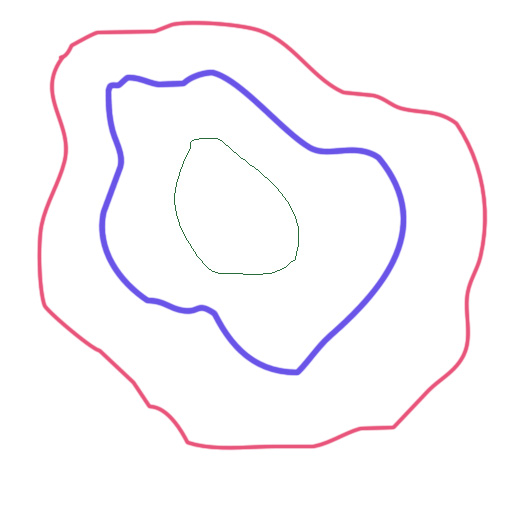
\includegraphics[width=0.65\textwidth,trim=3cm 8cm 0cm 0cm, clip]{tools/contours.png}\label{fig:tools-b}}\\
 \subfloat[Edge Detection (interactive GUI 
support for comparing different edge-detection algorithms)]{\includegraphics[width=0.6\textwidth]{tools/edge.png}\label{fig:tools-c}}\hspace*{1em}%
 \subfloat[Foreground/Background Probability (visualizing 
probability scalars and their combinations at different 
discretization levels)]{\includegraphics[width=0.44\textwidth,
trim=0cm 3cm 2cm 0cm, clip]{tools/trimap.png}\label{fig:tools-d}}\\
 \caption{GUI Tools for Interactive Image Processing}%
 \label{fig:tools-all}%
{\centerlabelbox{Screenshots of GUI components for interactive 
design or evaluation of Computer Vision workflows.\\Viewing 
color distributions and histograms [a], [b].  Comparing 
edge-detection algorithms [c].\\Visualizing 
foreground/background probabilities [d].}}
\end{figure*}


